\documentclass[a4paper, 12pt, oneside]{article}

\usepackage[a4paper,lmargin=4cm,rmargin=2cm,tmargin=2cm,bmargin=2cm]{geometry}
\usepackage[english]{babel}
\usepackage{amsmath}
\usepackage{graphicx}
\usepackage{caption}
\usepackage{subcaption}

\title{\large{MetaCortex contigs.fa}}

\begin{document}
\maketitle

\begin{figure}[h]
\centering
\begin{subfigure}[b]{0.45\textwidth}
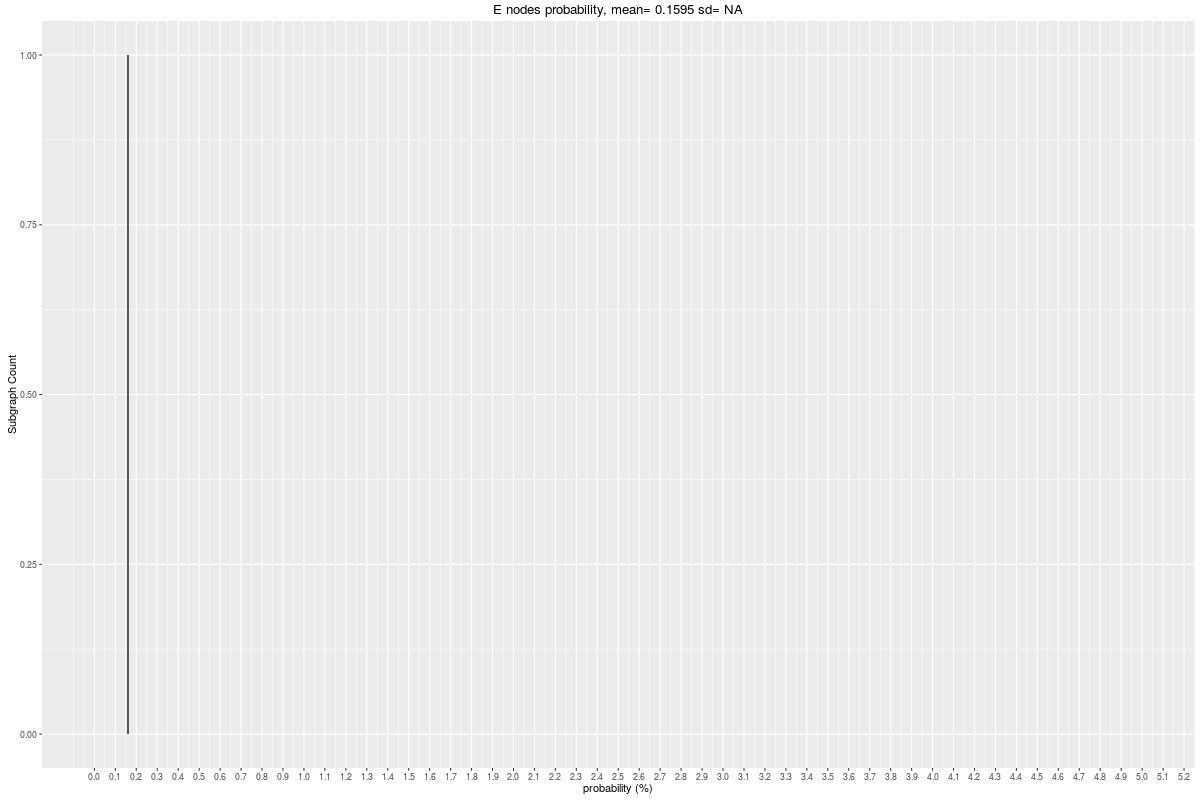
\includegraphics[width=\textwidth]{graphs/E_degrees.png}
\caption{\label{fig:E}E nodes}
\end{subfigure}
\begin{subfigure}[b]{0.45\textwidth}
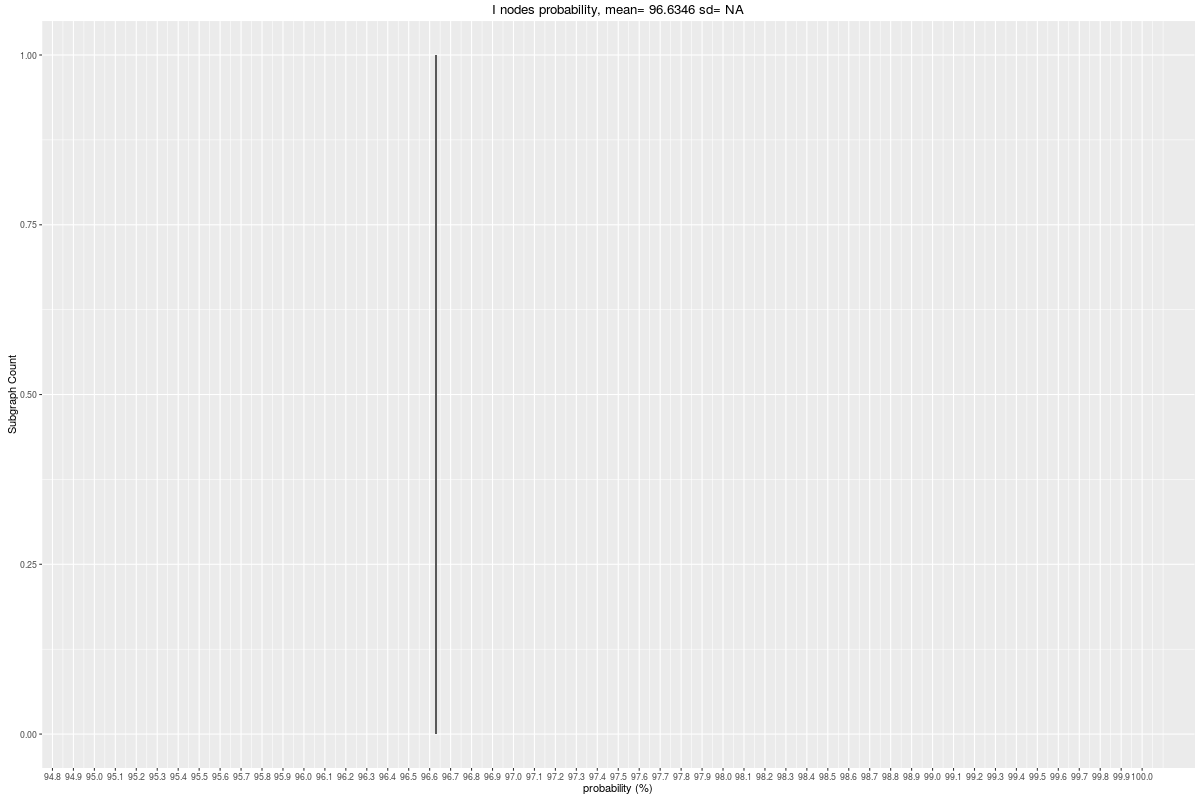
\includegraphics[width=\textwidth]{graphs/I_degrees.png}
\caption{\label{fig:I}I nodes }
\end{subfigure}
\begin{subfigure}[b]{0.45\textwidth}
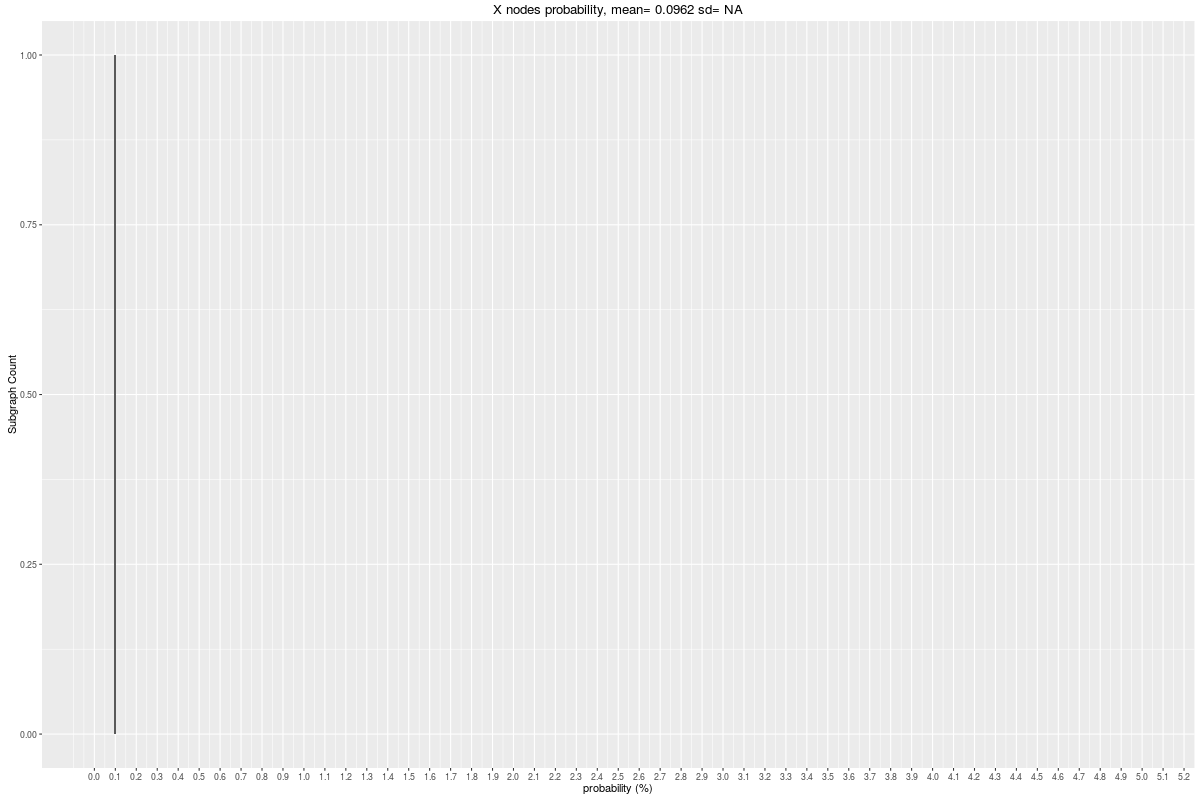
\includegraphics[width=\textwidth]{graphs/X_degrees.png}
\caption{\label{fig:X}X nodes}
\end{subfigure}
\begin{subfigure}[b]{0.45\textwidth}
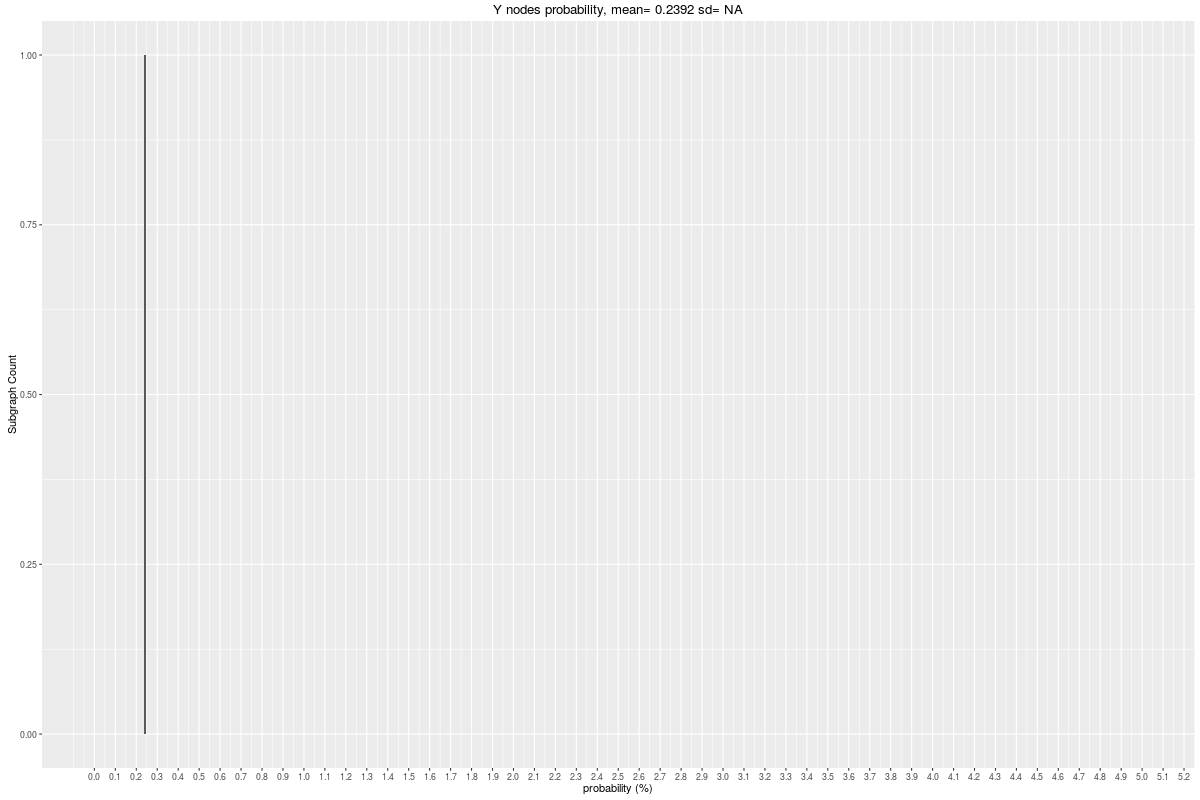
\includegraphics[width=\textwidth]{graphs/Y_degrees.png}
\caption{\label{fig:Y}Y nodes }
\end{subfigure}
\caption{Distribution of nodes in graph}\label{fig:E_and_I}
\end{figure}


\begin{figure}[h]
\centering
\begin{subfigure}[b]{0.45\textwidth}
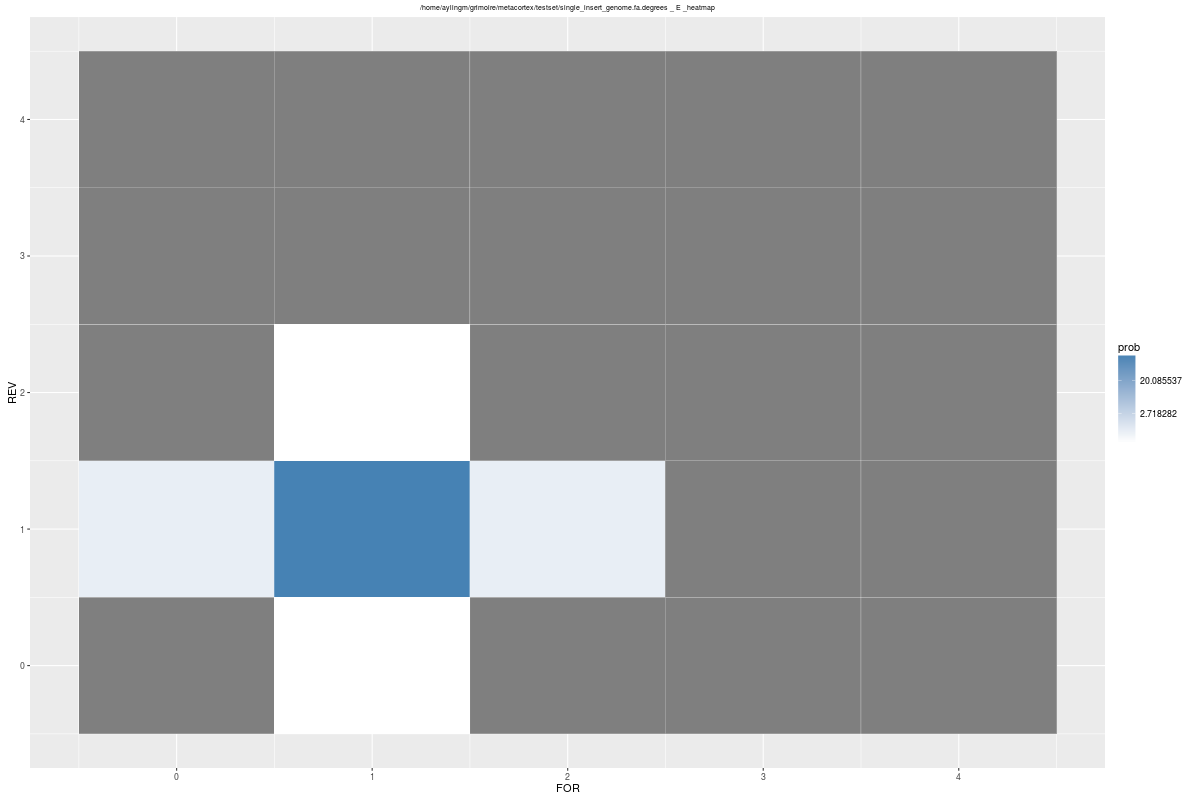
\includegraphics[width=\textwidth]{graphs/E_heatmap.png}
\caption{\label{fig:Heat}Heatmap of probability of node types}
\end{subfigure}
\begin{subfigure}[b]{0.45\textwidth}
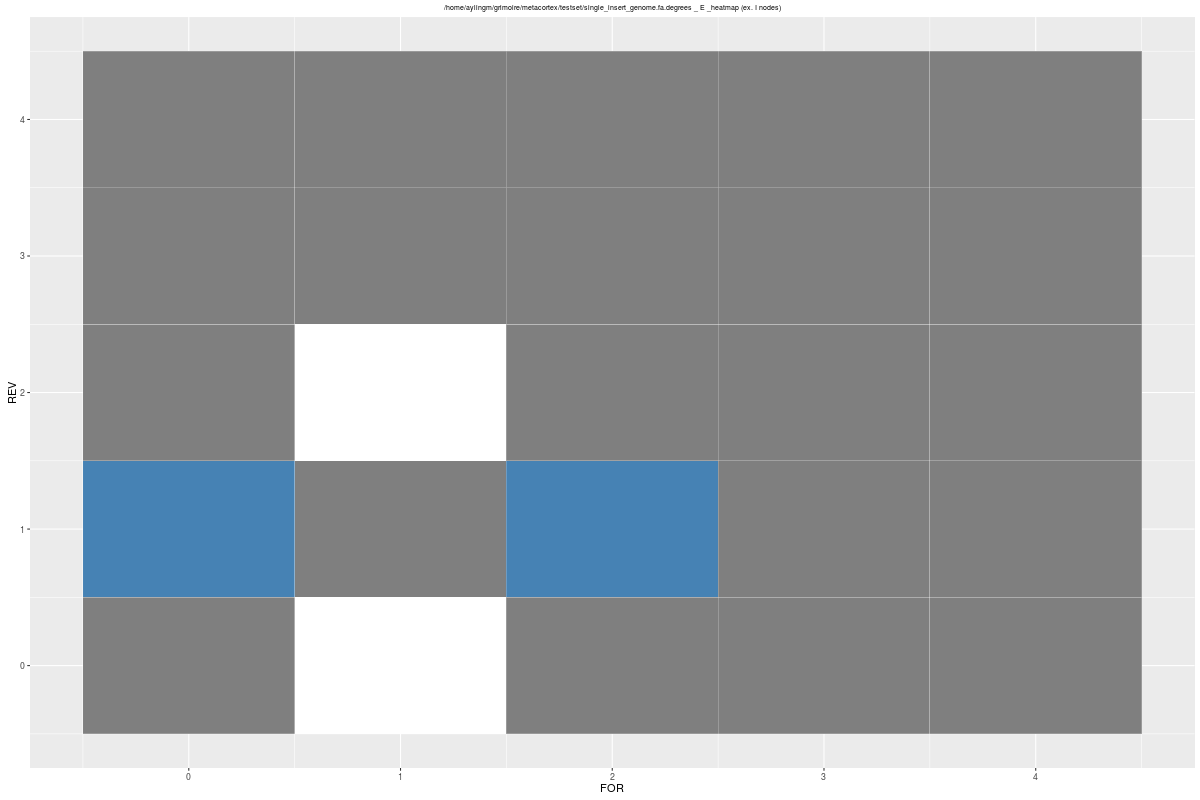
\includegraphics[width=\textwidth]{graphs/E_heatmap_noI.png}
\caption{\label{fig:Heat without I}Heatmap of probability of node types (with I nodes removed)}
\end{subfigure}
\caption{Heatmap of probability of nodes within the graph}\label{fig:E_and_I}
\end{figure}
\newpage

\textbf{Complexity distribution of total graph (X/Y nodes)}\\
0\quad 0\\
1\quad 0\\
2\quad 1\\
3\quad 0\\
4\quad 0\\

\textbf{Coverage dist}\\
1\quad 154\\
2-4\quad 47\\
\\
1\quad 154\\
2\quad 15\\
3\quad 32\\
4\quad 0\\
5\quad 0\\
6\quad 0\\
7\quad 0\\
8\quad 0\\
9\quad 0\\
\(\geq\)10   \quad 0\\
\\
\textbf{kmers}\\
unique\quad 201\quad\quad total\quad 400\quad\quad \% of total\quad 50.25\\
\\
\textbf{subgraphs}\\
largest subgraph\quad 201\quad\quad  \% of total\quad 100.00\\
num subgraphs\quad 1\quad num subgraphs\(>\)2k\quad 0\\
num subgraphs per E\textsuperscript{6} kmers\quad 0.004975\\
branches\quad 2\quad\quad per 1000 nodes\quad 0.00\\
\\
\textbf{graph size dist:}\\
\(\leq\)E\textsuperscript{0}\quad 0\\
\(\leq\)E\textsuperscript{1}\quad 0\\
\(\leq\)E\textsuperscript{2}\quad 1\\
\(\leq\)E\textsuperscript{3}\quad 0\\
\(\leq\)E\textsuperscript{4}\quad 0\\
\(\leq\)E\textsuperscript{5}\quad 0\\
\(\leq\)E\textsuperscript{6}\quad 0\\
\(\leq\)E\textsuperscript{7}\quad 0\\
\(\leq\)E\textsuperscript{8}\quad 0\\
\(\leq\)E\textsuperscript{9}\quad 0\\
\\
\textbf{highest coverage kmers}\\
3\quad ATAATATAAGAGAAATCGAAGGTATCATCAT\\
3\quad ACAAACAAAATACGGCAAAAAAATCGCGCAT\\
3\quad TACAAACAAAATACGGCAAAAAAATCGCGCA\\
3\quad ATACAAACAAAATACGGCAAAAAAATCGCGC\\
3\quad CATACAAACAAAATACGGCAAAAAAATCGCG\\
\\
\textbf{num simple graphs}\quad 0\\

\end{document}